\documentclass[tikz,border=8pt]{standalone}
\usepackage{amsmath,amssymb}
\usepackage{tikz}
\usepackage{pgfplots}
\pgfplotsset{compat=1.18}
\begin{document}
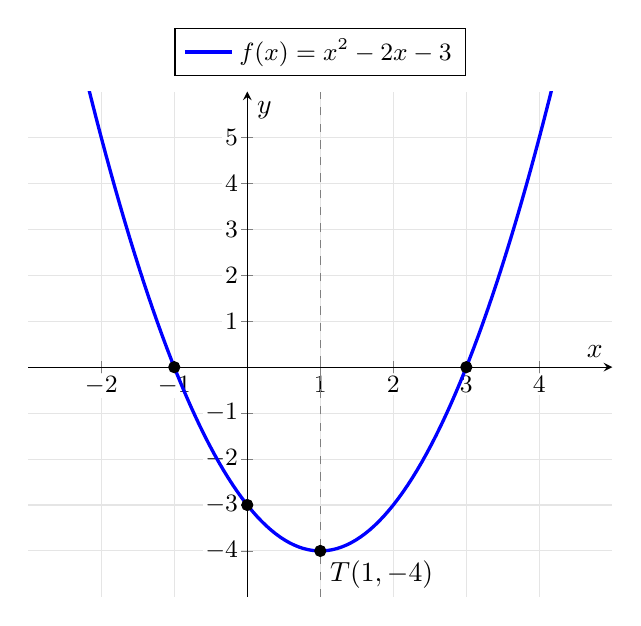
\begin{tikzpicture}
  \begin{axis}[
    axis lines=middle, xlabel={$x$}, ylabel={$y$},
    xmin=-3, xmax=5, ymin=-5, ymax=6,
    xtick={-2,-1,...,4}, ytick={-4,-3,...,5},
    grid=both, grid style={gray!20},
    width=9cm, height=8cm,
    legend style={font=\small, at={(0.5,1.03)}, anchor=south, legend columns=-1},
    every tick label/.append style={font=\small, fill=white, inner sep=1pt},
  ]
    \addplot[very thick, blue, domain=-2.2:4.2, samples=100] {x^2 - 2*x - 3};
    \addlegendentry{$f(x)=x^2-2x-3$}
    \addplot[dashed, gray, forget plot] coordinates {(1,-5) (1,6)};
    \addplot[only marks, mark=*, forget plot] coordinates {(-1,0) (3,0) (1,-4) (0,-3)};
    \node[below right] at (axis cs:1,-4) {$T(1,-4)$};
  \end{axis}
\end{tikzpicture}
\end{document}
